\section{微积分基本定理-下}\label{019}

\begin{tcolorbox}[size=fbox, breakable, enhanced jigsaw, title={更加严格的版本 - 选读}]

考虑一个在区间 \([a,b]\) 可积的 \(f(x)\), 和先前一样的, 令 \[
F(x):=\int_a^xf(\xi)\mathrm{d}\xi,
\] 这里 \(a\le x \le b\). 考虑 \(f(x)\) 在此区间的上下界, 若有
\(M\ge |f(x)|\) 在此区间内, 那么对于 \(a\le p \le q \le b\) 显然有 \[
|F(q)-F(p)|=\left|\int_p^qf(\xi)\mathrm{d}\xi\right|\le M\cdot(q-p).
\] (如果觉得不那么显然的话, 可以参考【\ref{018}\nameref{018}】``平均值''这一套论述).
于是对于 \(\epsilon>0\), 只要\(|q-p|<\epsilon/M\), 便有
\(|F(q)-F(p)|<\epsilon\), 这样首先证明了 \(F(x)\) 是连续的.

继而, 选定某个 \(x\), 且在此处 \(f(x)\) 是连续的. 给定 \(\epsilon>0\),
选择一个 \(\delta>0\), 使得若有 \(|\xi-x|<\delta\) 且 \(a\le\xi\le b\),
便有 \(|f(\xi)-f(x)|<\epsilon\).

如此一来, 如果 \(x-\delta<p\le x\le q<x+\delta\), 且 \(a\le p<q\le b\),
便有 \[
\begin{aligned}
\left|\frac{F(q)-F(p)}{q-p}-f(x)\right|&=\left|\frac{1}{q-p}\left(\int_a^qf(\xi)\mathrm{d}\xi-\int_a^pf(\xi)\mathrm{d}\xi\right)-f(x)\right|\\
&=\left|\frac{1}{q-p}\int_p^qf(\xi)\mathrm{d}\xi-f(x)\right|\\
&=\left|\frac{1}{q-p}\int_p^q[f(\xi)-f(x)]\mathrm{d}\xi\right|\\
&<\left|\frac{1}{q-p}\int_p^q\epsilon\mathrm{d}\xi\right|=\epsilon.
\end{aligned}
\] 也就是说, 在区间 \([a,b]\) 有 \(F'(x)=f(x)\). 以上我们用
\(\epsilon-\delta\) 语言更严格地证明了某种意义上, 积分和微分互为逆运算.

类似的, 尝试证明对于任意 \(\epsilon>0\) 都有
\(\left|F(b)-F(a)-\int_a^bf(x)\mathrm{d}x\right|<\epsilon\),
也可以严格证明定积分的微积分基本定理, 这一部分留作练习.

\end{tcolorbox}

\begin{tcolorbox}[size=fbox, breakable, enhanced jigsaw, title={应用? - 和物理的联系}]

经典的速度的定义是位移的导数,
\(v\equiv \frac{\mathrm{d}}{\mathrm{d}t}s(t)\).

如下图所示: 匀速的情况, 位移很好理解, 无非是速度乘上时间.
速度是阶梯函数的话, 位移依旧很好求, 分段计算即可.
若速度是连续变化的函数, 那么在我们有积分这个工具之前, 就非常困难了.

\begin{tcolorbox}[size=fbox, breakable, enhanced jigsaw]
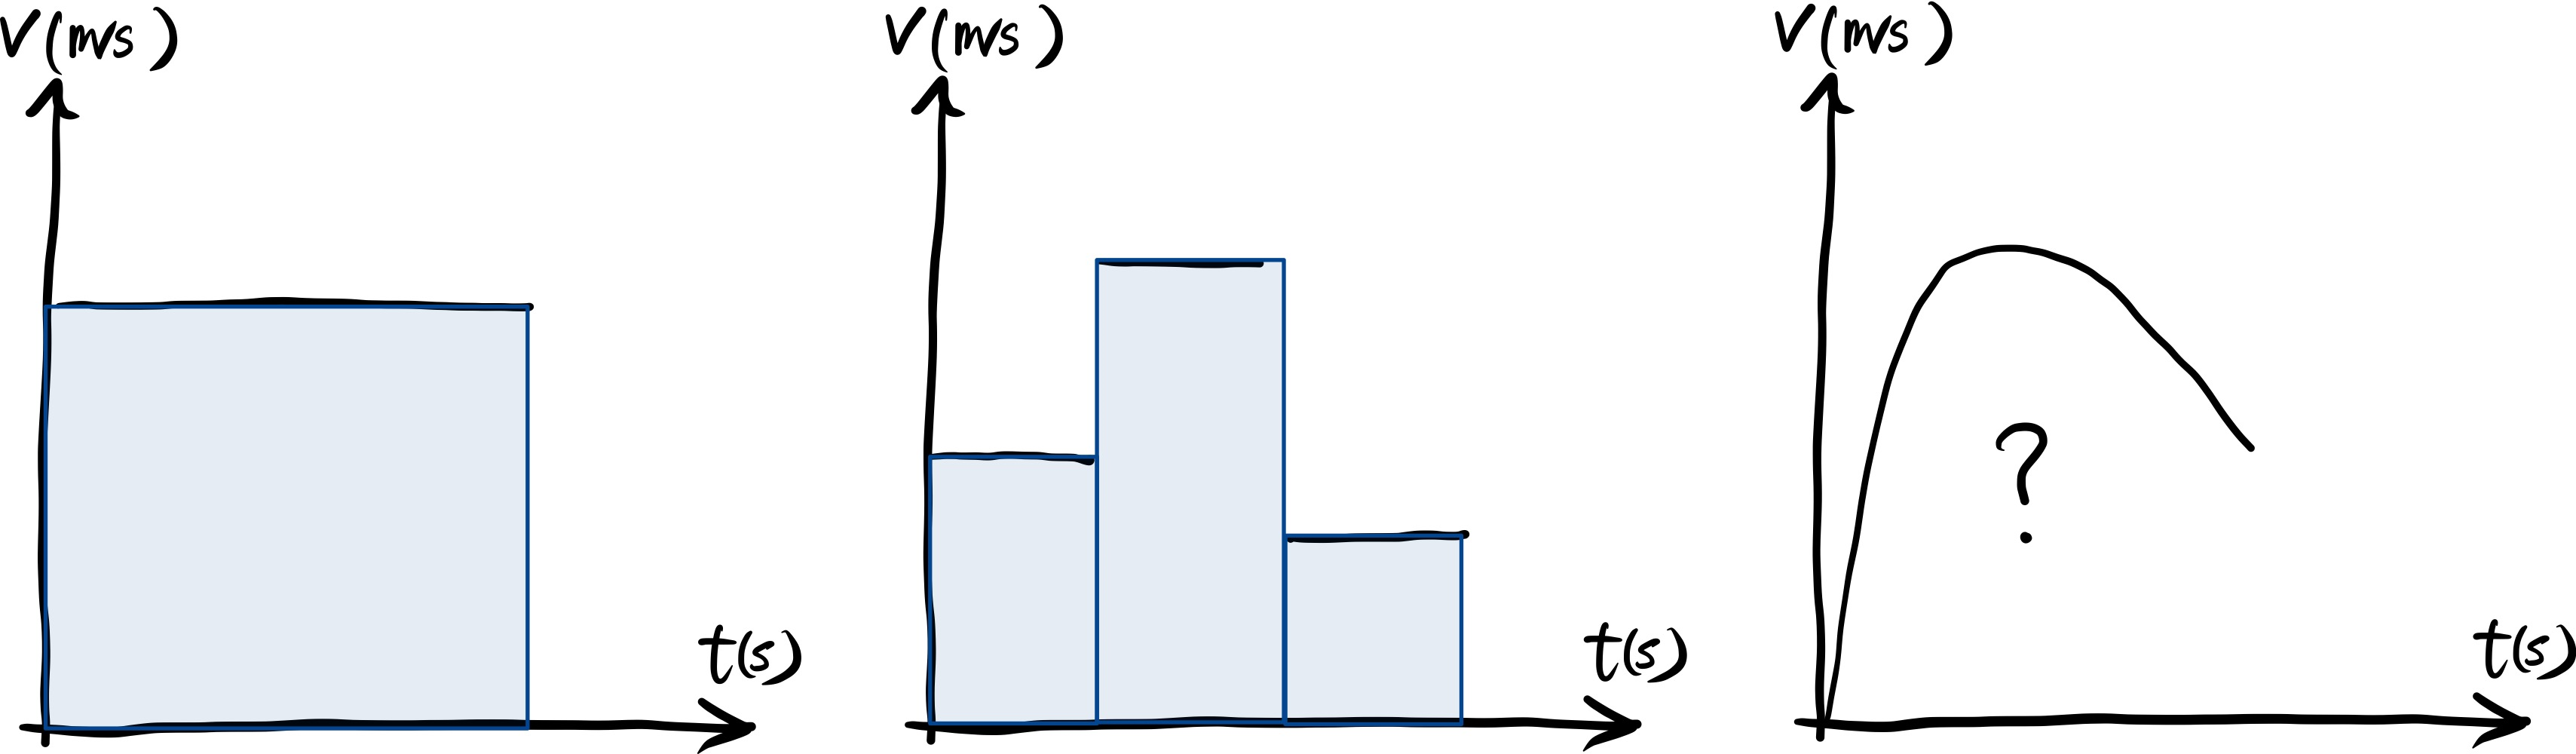
\includegraphics[width=0.9\textwidth]{img/image-20230912164801681.png}
\end{tcolorbox}

我们可以尝试将整个过程分成很多段, 每一段估计一个平均速度
(这一段时间内最大速度和最小速度之间的值), 然后把这一段近似成匀速计算,
或者将这一小段近似成匀变速的情况, 即 \(s=ut+\frac{1}{2}at^2\)
(如果没见过这个公式可以忽略它\ldots{} 不影响后面的理解). 不管怎么样,
对于匀速和速度是阶梯函数, 我们其实还是计算了\(v-t\)函数图像下的面积,
对于速度是连续函数的情况, 我们也还是在估算函数下方的面积, 于是很自然的,
若我们有积分这个工具, 速度又可以表示成一个关于时间的函数, 应该有 \[
s=\int v\mathrm{d}t.
\] 当然, 不定积分需要加上积分常数 (参见【\ref{018}\nameref{018}】文末),
这通常可以靠初始条件 (比如 \(t=0\) 时的位移) 来确定;
定积分反映的则是两个时间点之间发生的位移. 类似的,
既然加速度的定义是速度的变化率 (导数),
\(a\equiv \frac{\mathrm{d}}{\mathrm{d}t}v(t)\), 那么也应该有 \[
v=\int a\mathrm{d}t.
\] 当然, 也要注意不定积分需要用初始条件确定积分常数,
而不定积分反映的是两个时间点之间速度的变化量.

再还有很多情况:

\begin{itemize}
\item
  比如力时关于位置的一个函数, 那么做功就不再是简单的 \(W=Fx\), 而是
  \(W=\int F(x)\mathrm{d}x\) 了;
\item
  比如密度是关于位置的函数, 那么质量就不再是简单的 \(m=\rho V\), 而是
  \(m=\int \rho(\vec{r})\mathrm{d}V\), 这个体积微元 (volume
  differential/infinitesimal) 实际运算的时候需要计算三重积分, 即
  \(\int\cdot\mathrm{d}V=\iiint\cdot\mathrm{d}x\mathrm{d}y\mathrm{d}z=\iiint\cdot r^2\sin\theta\mathrm{d}r\mathrm{d}\theta\mathrm{d}\phi\),
  这里给的是三维直角坐标系和球状坐标系的例子,
  视情况和方便程度而定使用哪种坐标, 这里暂时不具体展开.
\end{itemize}
\end{tcolorbox}